\documentclass{article}
\usepackage{iclr2027_conference,times}
\usepackage[T1]{fontenc}
\usepackage{lmodern}
\usepackage{hyperref}
\usepackage{url}
\usepackage{booktabs}
\usepackage{microtype}
\usepackage{enumitem}
\usepackage{xcolor}
\usepackage{graphicx}
\usepackage{amsmath,amssymb}
\usepackage{amsthm}

\newtheorem{theorem}{Theorem}
\newtheorem{proposition}{Proposition}
\newtheorem{lemma}{Lemma}
\newtheorem{corollary}{Corollary}
\newtheorem{remark}{Remark}
\newcommand{\E}{\mathbb E}
\newcommand{\Pp}{\mathbb P}
\newcommand{\Var}{\operatorname{Var}}
\newcommand{\TV}{d_{\mathrm{TV}}}
\newcommand{\1}{\mathbf 1}
\newcommand{\Poi}{\operatorname{Poi}}
\newcommand{\Nstar}{N^\star}

\title{Closing the Harmonic Gap:\\
Exact Identity Testing for Zipfian Distributions}

\author{\textbf{Pahan Dewasurendra} \\ Johns Hopkins University}

\hypersetup{pdftitle={Closing the Harmonic Gap: Exact Identity Testing for Zipfian Distributions},pdfauthor={Pahan Dewasurendra},pdfkeywords={identity testing, distribution testing, Zipf distributions, instance optimality, sample complexity, exact constants},pdfsubject={preprint}}
\begin{document}
\maketitle

\begin{abstract}
Instance-optimal identity testing asks how many samples are needed to test an unknown discrete distribution against a specific known null. Existing characterizations truncate a constant multiple of the testing radius. This is usually harmless, but it creates a polynomial gap for the harmonic null $q_i\propto1/i$, the canonical obstruction highlighted in a 2024 COLT open problem. We give a constant-factor characterization for the full Zipfian class $q_i\asymp1/(Li)$. Let $m_q(\varepsilon)$ be the last index whose strict suffix has null mass at least $\varepsilon$. Throughout the nondegenerate range, \[ \Nstar(q,\varepsilon) =\Theta\!\left(L\sqrt{m_q(\varepsilon)} \max\{1,(\varepsilon L)^{-2}\}\right), \] where constants depend only on the fixed Zipf envelope. For the exact harmonic law, $L=H_k$ and $m_q(\varepsilon)=\Theta(k\exp(-\varepsilon H_k))$, so \[ \Nstar(q,\varepsilon) =\Theta\!\left(H_k\sqrt{k e^{-\varepsilon H_k}} \max\{1,(\varepsilon H_k)^{-2}\}\right). \] Thus, for every fixed $\varepsilon\in(0,1/3]$, the answer is $\Theta((\log k)k^{(1-\varepsilon)/2})$. The upper bound combines a coarsened instance-optimal test with one unweighted tail-collision statistic. Its key step is a water-filling inequality: if almost all of a Zipfian tail is deleted, its squared discrepancy cannot fall below the tail's collision mass. The lower bound introduces a graded-thinning prior. Tail coordinate $i$ is retained with probability proportional to $i^{-1/3}$ and inflated when retained. This profile makes the alternatives $\varepsilon$-far while keeping the mixture second moment bounded up to the matching sample size. Beyond settling the harmonic example robustly, the result isolates graded thinning as the mechanism missed by constant-radius truncations.
\end{abstract}

\section{Introduction}

Identity testing is the simplest distribution-testing problem with a nontrivial instance geometry. A known distribution $q$ on $[k]$ and samples from an unknown distribution $p$ are given. The goal is to distinguish $p=q$ from $\TV(p,q)>\varepsilon$. In the worst case over $q$, the optimal sample complexity is $\Theta(\sqrt{k}/\varepsilon^2)$ \citep{paninski2008coincidence,diakonikolas2018highprob}. For a fixed $q$, the answer can be much smaller. This motivates instance-optimal, also called massively parameterized, identity testing \citep{valiant2017automatic,goldreich2017property}.

The influential characterization of \citet{valiant2017automatic} uses the $\ell_{2/3}$ quasi-norm after removing the largest atom and a low-probability tail. Their lower and upper bounds remove, respectively, constant multiples of $\varepsilon$. \citet{blais2017distribution} give incomparable bounds in terms of the $K$-functional between $\ell_1$ and $\ell_2$. \citet{chhor2022sharp} characterize the dual local separation radius up to constants. None of these results gives a constant-factor sample complexity for every pair $(q,\varepsilon)$. The issue is not cosmetic. A constant change in the truncated mass can induce an arbitrarily large sample gap \citep{blais2017distribution,canonne2024open}.

The standard witness is the harmonic distribution \[ q^{(k)}_i=\frac{1}{iH_k},\qquad H_k=\sum_{j=1}^k\frac1j. \tag{1}\label{eq:harmonic} \] Removing tail mass $\varepsilon$ leaves about $k\exp(-\varepsilon H_k)=k^{1-\varepsilon+o(1)}$ coordinates. Hence a constant multiplying $\varepsilon$ changes a power of $k$. This example is the quantitative obstruction in the open problem of \citet{canonne2024open}.

We close this harmonic gap, and do so robustly for the Zipfian envelope $q_i\asymp1/(Li)$. The rate depends on the exact $\varepsilon$-tail quantile, so it preserves the accuracy rather than a constant multiple of it. The proof also explains why existing truncation arguments lose information. The hard alternatives do not perturb the retained head by a small symmetric amount. Instead, they thin the whole relevant tail at a coordinate-dependent rate and inflate the survivors. The best retention probability is proportional to the cube root of the null mass. Within a Zipf envelope this is equivalent to $(r/i)^{1/3}$ beyond a cutoff $r$.

\paragraph{Contributions.}
Our results are as follows.
\begin{enumerate}[leftmargin=*,itemsep=2pt,topsep=3pt]
\item We give a constant-factor sample complexity for every fixed Zipf
envelope $q_i\asymp1/(Li)$. The exact harmonic law is a corollary with universal constants. The answer transitions at $\varepsilon\asymp1/L$ from the classical quadratic-accuracy rate to an accuracy-dependent effective support.
\item We introduce a two-part tester. A standard identity test is applied to
a coarsening that preserves a head and lumps the tail. If it accepts, any far alternative must internally redistribute almost all of the tail. One unweighted collision statistic detects exactly this case.
\item We construct a matching graded-thinning prior and analyze it directly
in the fixed-sample multinomial experiment. Conditioning a single reservoir coordinate on a typical fluctuation enforces exact normalization without destroying the product second moment.
\item We prove quantitative water-filling and thinning lemmas that expose a
common cube-root profile on the algorithmic and information-theoretic sides.
\end{enumerate}

\section{Related work}

\paragraph{Identity and uniformity testing.}
Collision and chi-squared statistics yield the optimal $\sqrt{k}/\varepsilon^2$ worst-case rate \citep{goldreich2017property,canonne2020survey,canonne2022topics}. \citet{paninski2008coincidence} proved a sharp uniformity lower bound by a random perturbation prior. High-confidence identity testing is characterized by \citet{diakonikolas2018highprob}. We work at constant success probability and ask for the exact dependence on the known null.

\paragraph{Instance-optimal testing.}
\citet{valiant2017automatic} propose a weighted chi-squared statistic and show bounds based on a truncated $\ell_{2/3}$ quasi-norm. Their result is constant-factor sharp after allowing a constant rescaling of the testing radius. \citet{blais2017distribution} connect testing lower bounds to communication complexity and obtain a $K$-functional characterization, again with different constants at the radius. \citet{chhor2022sharp} study local minimax separation for multinomial, binomial, and Poisson experiments. A constant-factor separation radius does not invert to a constant-factor sample complexity when the radius occurs in an exponent. The open problem of \citet{canonne2024open} asks for a succinct functional that avoids this gap and singles out the harmonic distribution as the basic unresolved example. Our theorem resolves that example and its constant-factor Zipfian neighborhood, rather than the full arbitrary-null problem.

\paragraph{Lower-bound methods.}
Poissonization, random perturbations, and moment matching are standard tools for discrete testing \citep{paninski2008coincidence,valiant2017automatic}. Our lower prior differs from the symmetric perturbations used in prior instance-optimal bounds. It is a sparse, inhomogeneous thinning prior. Its retention profile is chosen to equalize the second-moment cost subject to deleting prescribed null mass.

\paragraph{Power-law nulls.}
Exponent-one Zipf laws are a standard model for ranked word frequencies, and discrete power-law profiles are a motivating structured family in distribution inference \citep{valiant2021chapter}. Previous instance-optimal testing guarantees still compare different constant multiples of the radius on this family. Our exact tail-quantile rate removes that ambiguity.

\section{Setup and main result}

For distributions $p,q$ on $[k]$, let \[ \TV(p,q)=\frac12\sum_{i=1}^k|p_i-q_i|. \] Let $\Nstar(q,\varepsilon)$ be the least integer $n$ for which a randomized test based on $n$ independent samples has both type-I error under $q$ and worst-case type-II error over $\{p:\TV(p,q)>\varepsilon\}$ at most $1/3$. Changing $1/3$ to another fixed constant changes all rates only by universal factors.

Fix $\kappa\geq1$. We call a nonincreasing null $q$ on $[k]$ $\kappa$-Zipfian if there is a scale $L$ such that \[ \frac{1}{\kappa Li}\leq q_i\leq\frac{\kappa}{Li} \qquad(i\in[k]).                                       \tag{2}\label{eq:zipfenvelope} \] Normalization implies $H_k/\kappa\leq L\leq\kappa H_k$. Define the exact tail quantile \[ m_q(\varepsilon)= \max\left(\{0\}\cup \left\{m\in[k-1]:\sum_{i>m}q_i\geq\varepsilon\right\}\right) \] and put $x=\varepsilon L$. The mild lower bound on $m_q(\varepsilon)$ below only excludes the endpoint where the effective tail has constant size.

\begin{theorem}[Zipfian identity testing]
\label{thm:main}
For every fixed $\kappa\geq1$, there are constants $c_\kappa,C_\kappa,r_\kappa>0$ such that every $\kappa$-Zipfian $q$ and every $0<\varepsilon\leq1/3$ with $m_q(\varepsilon)\geq r_\kappa$ satisfy \[ c_\kappa L\sqrt{m_q(\varepsilon)}\max\{1,x^{-2}\} \leq \Nstar(q,\varepsilon) \leq C_\kappa L\sqrt{m_q(\varepsilon)}\max\{1,x^{-2}\}. \tag{3}\label{eq:mainrate} \] The constants are independent of $k$, $q$, and $\varepsilon$.
\end{theorem}

\begin{corollary}[The harmonic gap]
\label{cor:fixed}
For $q^{(k)}$ in \eqref{eq:harmonic}, there are universal constants in \eqref{eq:mainrate} with $L=H_k$ and \[ m_q(\varepsilon)=\Theta(k e^{-\varepsilon H_k}). \] Consequently, for every fixed $\varepsilon\in(0,1/3]$, \[ \Nstar(q^{(k)},\varepsilon) =\Theta_\varepsilon\!\left((\log k)k^{(1-\varepsilon)/2}\right). \] The stronger statement \eqref{eq:mainrate} retains $\varepsilon$ inside the exponent with universal constants.
\end{corollary}

The factor $\max\{1,x^{-2}\}$ describes the transition. If $x\lesssim_\kappa1$, then $m_q(\varepsilon)=\Theta_\kappa(k)$ and \eqref{eq:mainrate} becomes \[ \Theta_\kappa\left(\frac{\sqrt{k}}{L\varepsilon^2}\right), \] the usual weighted chi-squared rate. Once $x$ is larger than a $\kappa$-dependent constant, the answer becomes $\Theta_\kappa(L\sqrt{m_q(\varepsilon)})$.

Table~\ref{tab:comparison} compares the fixed-accuracy consequences. We use the total-variation convention throughout. Constant changes between total variation and $\ell_1$ affect the displayed exponents in earlier bounds, so the entries state the constants as formulated by the cited results.

\begin{table}[t]
\centering
\small
\caption{Bounds for the harmonic null at fixed $\varepsilon$. Polynomial
factors in $k$ are shown explicitly.}
\label{tab:comparison}
\begin{tabular}{lll}
\toprule
Result & Type & Harmonic dependence, suppressing $\varepsilon$ constants\\
\midrule
Valiant--Valiant & lower &
$\Omega(k^{(1-\varepsilon)/2}/H_k)$\\
Blais--Canonne--Gur & lower &
$\Omega(k^{1/2-\varepsilon})$\\
Valiant--Valiant & upper &
$O(k^{(1-\varepsilon/16)/2}/H_k)$\\
Theorem~\ref{thm:main} & matching &
$\Theta(H_k k^{(1-\varepsilon)/2})$\\
\bottomrule
\end{tabular}
\end{table}

\begin{figure}[t]
\centering
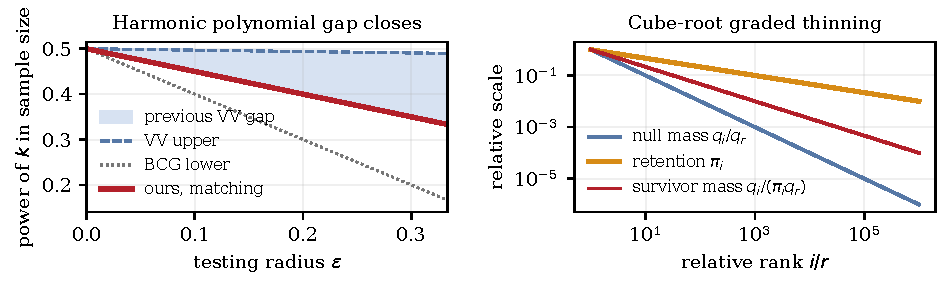
\includegraphics[width=\textwidth]{zipf_phase.pdf}
\caption{Left: for the harmonic null at fixed $\varepsilon$, previous
upper and lower bounds leave a polynomial range. Our matching rate lies on the sharp lower exponent and determines the missing logarithmic factor. Right: the hard prior retains rank $i$ with cube-root probability and inflates survivors, spreading its second-moment cost across the tail.}
\label{fig:phase}
\end{figure}

\section{The two-part upper bound}
\label{sec:upper}

We first give the new-regime proof. The standard small-$x$ tester is recalled at the end. Let $m=m_q(\varepsilon)$. Choose a sufficiently large constant $K_\kappa$, then put \[ r=\lfloor m/K_\kappa\rfloor, \qquad S=\{r+1,\ldots,k\}. \tag{4}\label{eq:cutoff} \] The Zipf envelope and the definition of $m$ imply \[ q(S)=\varepsilon+\Theta_\kappa(1/L),\quad \sum_{i\in S}q_i^2=O_\kappa(1/(L^2r)),\quad \|q_{[r]}\|_{2/3}=O_\kappa(\sqrt r/L). \tag{5}\label{eq:harmonicfacts} \] We choose $K_\kappa$ so that the first additive term in \eqref{eq:harmonicfacts} is positive and larger than the maximum atom.

The tester splits its samples into two independent batches.

\paragraph{Coarsened head test.}
Map every $i\in S$ to one new symbol $s$. Apply a standard instance-optimal identity test to the resulting distribution on $[r]\cup\{s\}$ at total-variation radius $\delta=c_\kappa/L$ for a small fixed $c_\kappa$. The tail cell has mass larger than $q_1$ and is the largest atom. Removing it leaves a vector whose full $\ell_{2/3}$ quasi-norm is $O_\kappa(\sqrt r/L)$. The upper bound of \citet{valiant2017automatic} therefore uses \[ O_\kappa\left(\frac{\sqrt r/L}{\delta^2}+\frac1\delta\right) =O_\kappa(L\sqrt r) \tag{6}\label{eq:headcost} \] samples.

\paragraph{Tail collision test.}
In a Poissonized batch with mean $n$, let $N_i$ be the count of symbol $i$ and compute \[ Z_S=\sum_{i\in S}\left((N_i-nq_i)^2-N_i\right). \tag{7}\label{eq:collision} \] Reject when $Z_S$ exceeds a sufficiently large constant threshold. Standard de-Poissonization changes the sample size by only a universal factor.

Why are these two tests enough? Put $\Delta=p-q$ and let $D_S=\sum_{i\in S}(-\Delta_i)_+$. If the coarsened distributions are within $\delta$, then \[ \sum_{i\leq r}|\Delta_i|+|\Delta(S)|<2\delta. \] Since the total negative discrepancy equals $\TV(p,q)$, every $\varepsilon$-far alternative satisfies \[ D_S\geq\varepsilon-2\delta. \tag{8}\label{eq:deleted} \] Thus all but $O_\kappa(1/L)$ of the null tail mass is deleted somewhere. The next lemma converts this one-sided statement into collision signal.

\begin{lemma}[Zipfian water filling]
\label{lem:waterfill}
Let $q$ satisfy \eqref{eq:zipfenvelope} and $S=\{r+1,\ldots,k\}$. Suppose $d_i\in[0,q_i]$ obey \[ \sum_{i\in S}d_i\geq q(S)-B/L. \] If $k/r\geq A_{\kappa,B}$, then \[ \sum_{i\in S}d_i^2\geq \frac{c_{\kappa,B}}{L^2r}, \qquad c_{\kappa,B}>0. \tag{9}\label{eq:waterfill} \]
\end{lemma}

The proof is a one-dimensional convex program. The minimizer is $d_i=\min\{q_i,\lambda\}$. The undeleted-mass budget and \eqref{eq:zipfenvelope} force the last uncapped index to be at most a $\kappa,B$-dependent multiple of $r$. Coordinates after it are fully deleted and their squared null mass is $\Omega_\kappa(1/(L^2r))$. Full details are in Appendix~\ref{app:waterfill}.

Apply Lemma~\ref{lem:waterfill} to $d_i=(-\Delta_i)_+$. Equations \eqref{eq:cutoff} and \eqref{eq:deleted} give, whenever the coarsened test has no signal, \[ A:=\sum_{i\in S}\Delta_i^2\geq c_\kappa/(L^2r). \tag{10}\label{eq:l2signal} \] Under Poisson sampling, \[ \E_p Z_S=n^2A, \quad \Var_p Z_S =2n^2\sum_{i\in S}p_i^2 +4n^3\sum_{i\in S}p_i\Delta_i^2. \tag{11}\label{eq:variance} \] The inequalities \[ \sum p_i^2\leq2\sum q_i^2+2A, \qquad \sum p_i\Delta_i^2 \leq q_{r+1}A+A^{3/2} \tag{12}\label{eq:variancebounds} \] show that $n=C_\kappa L\sqrt r$ makes the mean in \eqref{eq:variance} dominate its standard deviation. Under the null, $\E_qZ_S=0$ and $\Var_qZ_S=2n^2\sum_{i\in S}q_i^2=O_\kappa(1)$ after fixing the leading constant. Chebyshev's inequality completes the new-regime upper bound.

For $x$ below a fixed constant, apply the usual weighted identity tester directly to $q$. Its cost is $O_\kappa(\sqrt{k}/(L\varepsilon^2))$. This is within a $\kappa$-dependent factor of \eqref{eq:mainrate} on every bounded interval of $x$. Together with the two-part tester for larger $x$, it proves the upper half of Theorem~\ref{thm:main}.

\section{The graded-thinning lower bound}
\label{sec:lower}

The matching prior is easiest to describe using the same cutoff $r=\lfloor m_q(\varepsilon)/K_\kappa\rfloor$. For $i\in S$, let \[ \pi_i=(r/i)^{1/3}, \qquad Y_i\sim\operatorname{Bernoulli}(\pi_i) \tag{13}\label{eq:retention} \] independently. Set $A_i=Y_i/\pi_i-1$ and define a provisional tail by $p_i=q_i(1+A_i)=q_iY_i/\pi_i$. Coordinates $2,\ldots,r$ remain unchanged. Coordinate $1$ is a reservoir: \[ R=\sum_{i\in S}q_iA_i, \qquad p_1=q_1-R. \tag{14}\label{eq:reservoir} \] Every realization with $p_1\geq0$ is exactly normalized.

The deleted tail mass is \[ D=\sum_{i\in S}q_i(1-Y_i). \] The cube-root profile gives \[ \sum_{i\in S}q_i\pi_i\leq\frac{C_\kappa}{L}, \quad \Var(D)=O_\kappa(1/(L^2r)), \quad \Var(R)=O_\kappa(1/(L^2r)). \tag{15}\label{eq:concentration} \] The choice of $K_\kappa$ makes $q(S)-\varepsilon$ larger than the first term in \eqref{eq:concentration} by a fixed multiple of $1/L$. Thus the mean of $D$ exceeds $\varepsilon$ by $c_\kappa/L$. We condition on the event \[ \mathcal E=\left\{D>\varepsilon, |R|\leq\frac{B_\kappa}{L\sqrt r}\right\} \tag{16}\label{eq:event} \] for a fixed sufficiently large $B_\kappa$. If $r$ exceeds a $\kappa$-dependent constant, \eqref{eq:concentration} gives $\Pp(\mathcal E)\geq0.99$. Since $q_1\geq1/(\kappa L)$, also $p_1\geq0$ on $\mathcal E$.

Every conditioned realization is $\varepsilon$-far. Indeed, if $R<0$, the deleted tail mass $D$ is part of the total negative discrepancy. If $R\geq0$, the positive tail discrepancy is $D+R$. In both cases \[ \TV(p,q)\geq D>\varepsilon. \tag{17}\label{eq:far} \]

It remains to show that the mixture is indistinguishable. Let $p,p'$ be independent draws from the conditioned prior and let $L_p,L_{p'}$ be their likelihood ratios against $q$ for $n$ multinomial samples. The standard identity \[ \E_q[L_pL_{p'}] =\left(1+\sum_i\frac{(p_i-q_i)(p'_i-q_i)}{q_i}\right)^n \leq \exp\left(n\sum_i\frac{(p_i-q_i)(p'_i-q_i)}{q_i}\right) \tag{18}\label{eq:crossmoment} \] reduces the calculation to a bilinear form. The tail contribution factorizes before conditioning. The reservoir contribution is $O_\kappa(n/(Lr))$ on $\mathcal E$, which is $o(1)$ at the claimed scale.

\begin{lemma}[Thinning second moment]
\label{lem:thinning}
Let $A_i=Y_i/\pi_i-1$ with independent $Y_i\sim\operatorname{Bernoulli}(\pi_i)$ and $\pi_i=(r/i)^{1/3}$. If $A_i'$ is an independent copy, then for $n\leq c_\kappa L\sqrt r$, \[ \E\exp\left(n\sum_{i\in S}q_iA_iA_i'\right) \leq \exp(C_\kappa c_\kappa^2). \tag{19}\label{eq:thinningmoment} \] Here $C_\kappa$ depends only on the envelope. Moreover, $c_\kappa$ can be chosen so that the right-hand side is arbitrarily close to one.
\end{lemma}

The calculation behind Lemma~\ref{lem:thinning} is transparent. The centered multiplier has variance $v_i=(1-\pi_i)/\pi_i$. A scalar Taylor bound gives \[ \log\E e^{nq_iA_iA_i'}\leq Cn^2q_i^2v_i^2, \] uniformly because $nq_i\max\{1,v_i^2\}=O_\kappa(r^{-1/2})$. Finally, \[ \sum_{i\in S}q_i^2v_i^2 \leq \sum_{i\in S}\frac{q_i^2}{\pi_i^2} =O_\kappa(1/(L^2r)). \tag{20}\label{eq:secondcost} \]

Conditioning costs at most $\Pp(\mathcal E)^{-2}$ in the positive second-moment integral. Combining \eqref{eq:crossmoment}, \eqref{eq:event}, and Lemma~\ref{lem:thinning}, then choosing $c_\kappa$ small and $r_\kappa$ large, shows that the chi-squared divergence between the null sample law and the mixture is below a fixed small constant. Le Cam's method proves \[ \Nstar(q,\varepsilon)=\Omega_\kappa(L\sqrt r) =\Omega_\kappa(L\sqrt{m_q(\varepsilon)}). \tag{21}\label{eq:newlower} \]

When $x\lesssim_\kappa1$, the classical Valiant--Valiant perturbation bound gives \[ \Omega_\kappa\left(\frac{\sqrt{k}}{L\varepsilon^2}\right) =\Omega_\kappa\left(L\sqrt{m_q(\varepsilon)}\,x^{-2}\right). \tag{22}\label{eq:smalllower} \] For $x$ larger than a constant, \eqref{eq:newlower} dominates. Equations \eqref{eq:newlower} and \eqref{eq:smalllower} prove the lower half of Theorem~\ref{thm:main}. Appendix~\ref{app:lower} supplies all constants and the conditioning argument.

\section{Why the cube root appears}
\label{sec:interpretation}

The lower prior gives a simple variational explanation. Suppose a tail coordinate is retained with probability $\pi_i$ and inflated by $1/\pi_i$. Its leading mixture cost is $q_i^2/\pi_i^2$, while its expected undeleted null mass is $q_i\pi_i$. Minimizing \[ \sum_i\frac{q_i^2}{\pi_i^2} \quad\text{subject to}\quad \sum_iq_i\pi_i\leq b \tag{23}\label{eq:variational} \] gives $\pi_i\propto q_i^{1/3}$ by the Lagrange equations. For $q_i\propto1/i$, this is precisely \eqref{eq:retention}.

There is a parallel cube-root law in the head. The weighted chi-squared tester uses $q_i^{-2/3}$, and its complexity is governed by the $\ell_{2/3}$ quasi-norm. The head and tail are therefore not unrelated proof cases. They are the small-perturbation and sparse-thinning faces of the same optimization. Constant-radius truncation captures the first face but discards the graded structure of the second.

This observation suggests a route toward the full open problem. A general functional must interpolate between symmetric perturbation cost $q_i^2a_i^4$ for small relative changes $a_i$ and thinning cost $q_i^2/(1-a_i)^2$ as deletion approaches one. Proving a matching tester for arbitrary, non-Zipfian nulls remains open. Our collision argument works for the full envelope \eqref{eq:zipfenvelope} because water filling changes an index cutoff only by a $\kappa$-dependent factor.

\section{Limitations and conclusion}

Theorem~\ref{thm:main} resolves the canonical harmonic instance and a robust constant-factor Zipfian class, but it does not characterize every null. The stated range $\varepsilon\leq1/3$ avoids a finite-support endpoint in which only constantly many leading coordinates remain. The techniques can cover a larger range with additional boundary cases, but that would obscure the accuracy-sensitive phenomenon.

The main conclusion is that a low-mass tail cannot always be ignored. When its mass is only $O_\kappa(1/L)$ above the testing radius, the hardest alternatives redistribute that tail through graded thinning. A coarsened head test and one collision statistic recover the missing upper bound, while the same cube-root profile yields a matching lower prior. This closes the polynomial harmonic gap throughout its natural envelope and identifies a concrete ingredient that any full instance-optimal characterization must represent.

\bibliography{references}
\bibliographystyle{iclr2027_conference}

\appendix
\section{Zipf-envelope estimates}
\label{app:harmonic}

We collect the finite-sum estimates used in the proof. For integers
$1\leq a<b$,
\begin{align}
 \log\frac{b+1}{a+1}
 &\leq \sum_{i=a+1}^b\frac1i
 \leq \log\frac ba,                                      \tag{24}\label{eq:hsum}\\
 \frac{1}{b+1}
 &\leq \sum_{i=b+1}^{\infty}\frac1{i^2}
 \leq \frac1b.                                           \tag{25}\label{eq:squaresum}
\end{align}
More generally, for $\alpha>1$,
\[
 \sum_{i=a+1}^{\infty}i^{-\alpha}
 \leq \int_a^\infty t^{-\alpha}\,dt
 =\frac{a^{1-\alpha}}{\alpha-1}.                         \tag{26}\label{eq:pseries}
\]
The reverse bound with $a+1$ in place of $a$ follows by the same
integral comparison.

Let $q$ satisfy \eqref{eq:zipfenvelope}, put
$m=m_q(\varepsilon)$, and let $r=\lfloor m/K_\kappa\rfloor$. Maximality
of $m$ gives
\[
 \varepsilon\leq q(\{m+1,\ldots,k\})
 <\varepsilon+\frac{\kappa}{L(m+1)}.
\]
Applying \eqref{eq:hsum} between $r$ and $m$, and choosing the fixed
$K_\kappa$ sufficiently large, gives constants
$0<b_\kappa<B_\kappa<\infty$ such that
\[
 \varepsilon+\frac{b_\kappa}{L}
 \leq q(\{r+1,\ldots,k\})
 \leq \varepsilon+\frac{B_\kappa}{L}.                  \tag{27}\label{eq:tailmassbounds}
\]
Also,
\[
 \frac{c_\kappa}{L^2r}
 \leq\sum_{i=r+1}^kq_i^2
 \leq\frac{C_\kappa}{L^2r},                             \tag{28}\label{eq:tailcollisionbounds}
\]
provided $k/r$ exceeds a $\kappa$-dependent constant. Finally,
\begin{align}
 \sum_{i=1}^r q_i^{2/3}
 &=\Theta_\kappa(L^{-2/3}r^{1/3}),\nonumber\\
 \|q_{[r]}\|_{2/3}
 &=\left(\sum_{i=1}^r q_i^{2/3}\right)^{3/2}
 =\Theta_\kappa(\sqrt r/L).                             \tag{29}\label{eq:headnorm}
\end{align}
Here and below $\|z\|_{2/3}=(\sum_i|z_i|^{2/3})^{3/2}$.

For the exact harmonic law, \eqref{eq:hsum} and maximality of $m$ give
\[
 \log(k/m)=\varepsilon H_k+O(1),
\]
uniformly in the nondegenerate range. Hence
$m=\Theta(k e^{-\varepsilon H_k})$, proving the tail-quantile assertion
in Corollary~\ref{cor:fixed}.

\section{The water-filling lemma}
\label{app:waterfill}

We prove Lemma~\ref{lem:waterfill} in a slightly more explicit form.

\begin{lemma}[Capped quadratic minimization]
\label{lem:capped}
Let $u_1\geq u_2\geq\cdots\geq u_M>0$ and $0<a<\sum_i u_i$.
The minimizer of
\[
 \min\left\{\sum_{i=1}^M d_i^2:
 0\leq d_i\leq u_i,\ \sum_i d_i\geq a\right\}
\]
has the form $d_i=\min\{u_i,\lambda\}$ for a unique $\lambda>0$.
\end{lemma}

\begin{proof}
The inequality constraint is tight at a minimizer. Strict convexity gives
uniqueness. The Karush--Kuhn--Tucker conditions state that every coordinate
strictly below its cap has the same value $\lambda$, while a coordinate at
its cap has $u_i\leq\lambda$. This is exactly the claimed form.
\end{proof}

\begin{proof}[Proof of Lemma~\ref{lem:waterfill}]
It is enough to impose equality
$\sum_{i\in S}d_i=q(S)-B/L$. Apply Lemma~\ref{lem:capped} with
$u_i=q_i$. Let $t$ be the last index for which $q_t>\lambda$. Up to
rounding, the minimizer is
\[
 d_i=\lambda\quad(r<i\leq t),
 \qquad d_i=q_i\quad(i>t).                               \tag{30}\label{eq:waterform}
\]
The undeleted mass is at most $B/L$. If $t>r$, then the Zipf envelope and
$\lambda<q_t\leq\kappa/(Lt)$ give
\begin{align*}
 \frac{B}{L}
 &\geq\sum_{i=r+1}^{\lfloor t\rfloor}(q_i-\lambda)\\
 &\geq\frac1{\kappa L}
   \log\frac{\lfloor t\rfloor+1}{r+1}-\frac{\kappa}{L}.
\end{align*}
For $r$ above a $\kappa,B$-dependent constant this implies
$t\leq A_{\kappa,B}'r$. If $t\leq r$, then $d_i=q_i$ throughout $S$,
and \eqref{eq:tailcollisionbounds} gives the result directly. Otherwise,
choose $A_{\kappa,B}\geq2A_{\kappa,B}'$. The assumption
$k/r\geq A_{\kappa,B}$ ensures that $\{t+1,\ldots,2t\}$ is available.
By \eqref{eq:waterform}, \eqref{eq:zipfenvelope}, and
\eqref{eq:squaresum},
\[
 \sum_{i\in S}d_i^2
 \geq\sum_{i>t}q_i^2
 \geq\frac{c_\kappa}{L^2(t+1)}
 \geq\frac{c_{\kappa,B}}{L^2r}.
\]
This proves the claim.
\end{proof}

\section{Details of the upper bound}
\label{app:upper}

We first record the statistic calculation.

\begin{lemma}[Poisson collision moments]
\label{lem:poissonmoments}
Let $N_i\sim\Poi(np_i)$ independently, let $\Delta_i=p_i-q_i$, and let
\[
 Z_T=\sum_{i\in T}\big((N_i-nq_i)^2-N_i\big).
\]
Then
\begin{align}
 \E_pZ_T&=n^2\sum_{i\in T}\Delta_i^2,                    \tag{31}\label{eq:zmean}\\
 \Var_pZ_T&=2n^2\sum_{i\in T}p_i^2
 +4n^3\sum_{i\in T}p_i\Delta_i^2.                       \tag{32}\label{eq:zvar}
\end{align}
\end{lemma}

\begin{proof}
For $N\sim\Poi(\lambda)$, the first four factorial moments give
\[
 \E[(N-a)^2-N]=(\lambda-a)^2
\]
and
\[
 \Var((N-a)^2-N)=2\lambda^2+4\lambda(\lambda-a)^2.
\]
Set $\lambda=np_i$ and $a=nq_i$, then sum independent coordinates.
\end{proof}

\begin{lemma}[Tail collision test]
\label{lem:tailtest}
Let $S=\{r+1,\ldots,k\}$ and suppose
\[
 \sum_{i\in S}q_i^2\leq\frac{C_0}{L^2r},\quad
 q_{r+1}\leq\frac{C_0}{Lr}.
\]
There is a constant $C=C(C_0,c_0)$ such that, using a Poissonized sample with
$n=CL\sqrt r$, one can distinguish $p=q$ from
\[
 \sum_{i\in S}(p_i-q_i)^2\geq\frac{c_0}{L^2r}
\]
with both errors at most $1/12$.
\end{lemma}

\begin{proof}
Put $A=\sum_{i\in S}\Delta_i^2$ and
$Q_2=\sum_{i\in S}q_i^2$. Besides
$\sum p_i^2\leq2Q_2+2A$, we have
\begin{align*}
 \sum_{i\in S}p_i\Delta_i^2
 &\leq\sum_{i\in S}(q_i+|\Delta_i|)\Delta_i^2\\
 &\leq q_{r+1}A+\sum_{i\in S}|\Delta_i|^3\\
 &\leq q_{r+1}A+A^{3/2}.
\end{align*}
The last step is monotonicity of finite-dimensional norms.

Let $A_0=c_0/(L^2r)$ and reject when
$Z_S>n^2A_0/2$. Under the null, Lemma~\ref{lem:poissonmoments} and
$Q_2=O(A_0)$ show that the rejection probability is $O(C^{-2})$.
Under an alternative with $A\geq A_0$, the squared ratio of the standard
deviation to the mean is at most
\[
 O\left(
 \frac{Q_2+A}{n^2A^2}
 +\frac{q_{r+1}}{nA}
 +\frac1{n\sqrt A}
 \right)=O(C^{-1}).                                      \tag{33}\label{eq:snrbound}
\]
Choosing $C$ sufficiently large and applying Chebyshev's inequality proves
the lemma.
\end{proof}

We now assemble the new-regime algorithm. Coarsen $q$ by preserving
$1,\ldots,r$ and replacing $S$ by a single cell. Call the coarsened null
$\bar q$. By \eqref{eq:tailmassbounds}, the tail cell is the largest cell.
The general upper bound of \citet[Theorem 2]{valiant2017automatic}, applied
at radius $\delta=c_\kappa/L$ for a sufficiently small fixed
$c_\kappa$, is at most
\[
 C_\kappa\max\left\{\delta^{-1},
 \frac{\|\bar q_{-\max}\|_{2/3}}{\delta^2}\right\}
 \leq C_\kappa'L\sqrt r,                                \tag{34}\label{eq:coarsebound}
\]
where using the untruncated quasi-norm only enlarges the published upper
bound. Equation \eqref{eq:headnorm} gives the last inequality.

Suppose $\TV(p,q)>\varepsilon$ and
$\TV(\bar p,\bar q)<\delta$. Since
\[
 2\TV(\bar p,\bar q)
 =\sum_{i\leq r}|p_i-q_i|+|p(S)-q(S)|,
\]
the total negative discrepancy outside $S$ is below $2\delta$. Therefore
\[
 \sum_{i\in S}(q_i-p_i)_+
 \geq\varepsilon-2\delta.                               \tag{35}\label{eq:tailnegative}
\]
By \eqref{eq:tailmassbounds}, the right side of
\eqref{eq:tailnegative} is at least $q(S)-B_\kappa'/L$. Moreover,
$q(\{m+1,\ldots,k\})\leq(\kappa/L)\log(k/m)$, so
$k/r\geq K_\kappa e^{x/\kappa}$. For $x$ above a
$\kappa$-dependent constant, Lemma~\ref{lem:waterfill} with
$B=B_\kappa'$ gives
\[
 \sum_{i\in S}(p_i-q_i)^2
 \geq\sum_{i\in S}(q_i-p_i)_+^2
 \geq\frac{c_\kappa}{L^2r}.                             \tag{36}\label{eq:tailsignalappendix}
\]
Lemma~\ref{lem:tailtest} detects this alternative. Splitting samples and
amplifying each component test to error $1/12$ gives total error below
$1/3$.

For $x$ below that fixed $\kappa$-dependent constant, the untruncated
version of the same Valiant--Valiant upper bound
uses
\[
 O_\kappa\left(\frac{\|q\|_{2/3}}{\varepsilon^2}\right)
 =O_\kappa\left(\frac{\sqrt k}{L\varepsilon^2}\right)
 =O_\kappa\left(L\sqrt{m_q(\varepsilon)}
     \max\{1,x^{-2}\}\right),                         \tag{37}\label{eq:smallupperappendix}
\]
because \eqref{eq:zipfenvelope} gives
$m_q(\varepsilon)=\Theta_\kappa(k)$ whenever $x$ stays bounded.

The argument above uses Poissonized samples only for the collision statistic.
The standard comparison between multinomial and Poisson experiments gives a
fixed-sample tester at constant overhead. Concretely, given $2n$ observations,
draw $M\sim\Poi(n)$ independently. If $M\leq2n$, use the first $M$
observations. Without the truncation, their cell counts are independent
$\Poi(np_i)$ variables. The event $M>2n$ is exponentially unlikely, so adding
it to the error budget changes only the universal constant.

\section{Details of the thinning lower bound}
\label{app:lower}

We prove the concentration and second-moment statements from
Section~\ref{sec:lower}. Recall that $S=\{r+1,\ldots,k\}$,
$\pi_i=(r/i)^{1/3}$, $Y_i\sim\operatorname{Bernoulli}(\pi_i)$, and
$A_i=Y_i/\pi_i-1$.

\subsection{The alternatives are valid and far}

Integral comparison gives
\begin{align}
 \sum_{i\in S}q_i\pi_i
 &\leq\frac{\kappa r^{1/3}}{L}\sum_{i>r}i^{-4/3}
 \leq\frac{3\kappa}{L},                                  \tag{38}\label{eq:retainedmass}\\
 \Var(D)
 &\leq\sum_{i\in S}q_i^2\pi_i
 \leq\frac{C_\kappa}{L^2r},                             \tag{39}\label{eq:dvar}\\
 \Var(R)
 &=\sum_{i\in S}q_i^2\frac{1-\pi_i}{\pi_i}
 \leq\sum_{i\in S}\frac{q_i^2}{\pi_i}
 \leq\frac{C_\kappa}{L^2r}.                             \tag{40}\label{eq:rvar}
\end{align}
The exponents in the last two sums are $7/3$ and $5/3$, respectively.
By \eqref{eq:tailmassbounds} and \eqref{eq:retainedmass},
\[
 \E D=q(S)-\sum_{i\in S}q_i\pi_i
 \geq\varepsilon+c_\kappa/L.                            \tag{41}\label{eq:dmargin}
\]

Fix $B_\kappa$ so that $C_\kappa/B_\kappa^2\leq1/400$.
Chebyshev's inequality yields
\begin{align*}
 \Pp(D\leq\varepsilon)&\leq C_\kappa/r,\\
 \Pp\left(|R|>B_\kappa/(L\sqrt r)\right)&\leq1/400.
\end{align*}
For a $\kappa$-dependent $r_\kappa$, the event $\mathcal E$ in
\eqref{eq:event} has probability $\alpha\geq0.99$. Increasing
$r_\kappa$ ensures $B_\kappa/\sqrt r<1/\kappa$, hence
$p_1=q_1-R>0$ on $\mathcal E$.

For completeness, let $U$ be the positive tail discrepancy. Since
$R=U-D$, if $R<0$ then the total negative discrepancy is $D$. If
$R\geq0$, the reservoir contributes negative discrepancy $R$ and the
total negative discrepancy is $D+R=U$. Thus $\TV(p,q)\geq D$ in both
cases. Every conditioned alternative is valid and more than
$\varepsilon$ away from $q$.

\subsection{A scalar cross-moment bound}

\begin{lemma}[Centered Bernoulli multiplier]
\label{lem:scalar}
Let $Y,Y'$ be independent $\operatorname{Bernoulli}(\pi)$ variables,
let $A=Y/\pi-1$, and let $A'$ be its independent copy. Put
$v=(1-\pi)/\pi$. If
\[
 |t|\max\{1,v^2\}\leq\frac12,
\]
then
\[
 \E e^{tAA'}\leq\exp(Ct^2v^2)                           \tag{42}\label{eq:scalarbound}
\]
for a universal constant $C$.
\end{lemma}

\begin{proof}
The variable $A$ takes values $-1$ and $v$, has mean zero, and satisfies
$\E A^2=v$. Consequently, $X=AA'$ has mean zero,
$\E X^2=v^2$, and $|X|\leq\max\{1,v^2\}$. Taylor's theorem and the
assumption give
\[
 e^{tX}\leq1+tX+C t^2X^2.
\]
Taking expectations and using $1+z\leq e^z$ proves the result.
\end{proof}

\begin{proof}[Proof of Lemma~\ref{lem:thinning}]
Let $t_i=nq_i$ and $v_i=(1-\pi_i)/\pi_i$. If
$n\leq c_\kappa L\sqrt r$, then for every $i>r$,
\begin{align*}
 t_i&\leq c_\kappa\kappa\sqrt r/i
       \leq c_\kappa\kappa/\sqrt r,\\
 t_iv_i^2&\leq t_i/\pi_i^2
 \leq c_\kappa\kappa r^{-1/6}i^{-1/3}
       \leq c_\kappa\kappa/\sqrt r.
\end{align*}
Thus Lemma~\ref{lem:scalar} applies for a sufficiently small
$c_\kappa$ and large $r$. Independence across coordinates gives
\begin{align*}
 \log\E\exp\left(n\sum_{i\in S}q_iA_iA_i'\right)
 &\leq Cn^2\sum_{i\in S}q_i^2v_i^2\\
 &\leq\frac{C_\kappa n^2}{L^2r^{2/3}}
       \sum_{i>r}i^{-4/3}\\
 &\leq\frac{C_\kappa'n^2}{L^2r}
 \leq C_\kappa'c_\kappa^2.
\end{align*}
This proves \eqref{eq:thinningmoment}.
\end{proof}

\subsection{Conditioning and the fixed-sample experiment}

Let $\mu$ be the prior conditioned on $\mathcal E$ and let $M_n$ be the
resulting mixture law of $n$ independent observations. For two valid
alternatives $p,p'$ drawn from $\mu$, the multinomial likelihood-ratio
identity is
\[
 \E_{q^{\otimes n}}L_pL_{p'}
 =\left(\sum_{i=1}^k\frac{p_ip_i'}{q_i}\right)^n
 =\left(1+\sum_{i=1}^k\frac{\Delta_i\Delta_i'}{q_i}\right)^n.
 \tag{43}\label{eq:multicross}
\]
The base in \eqref{eq:multicross} is nonnegative. Using
$1+z\leq e^z$, equations \eqref{eq:reservoir} and
\eqref{eq:event} give
\begin{align}
 1+\chi^2(M_n,q^{\otimes n})
 &\leq\E_{p,p'\sim\mu}
 \exp\left(n\sum_{i\in S}q_iA_iA_i'+n\frac{RR'}{q_1}\right)\nonumber\\
 &\leq \exp\left(\frac{\kappa nB_\kappa^2}{Lr}\right)
 \alpha^{-2}
 \E\exp\left(n\sum_{i\in S}q_iA_iA_i'\right).           \tag{44}\label{eq:conditionedmoment}
\end{align}
The last expectation is under the unconditioned product prior. The factor
$\alpha^{-2}$ follows by dropping two indicators from a nonnegative
integrand.

Set $n=c_\kappa L\sqrt r$. Lemma~\ref{lem:thinning} and
\eqref{eq:conditionedmoment} imply
\[
 1+\chi^2(M_n,q^{\otimes n})
 \leq \exp(c_\kappa\kappa B_\kappa^2/\sqrt r)
       \alpha^{-2}\exp(C_\kappa c_\kappa^2).
 \tag{45}\label{eq:finalchi}
\]
Choose $r_\kappa$ large and then $c_\kappa$ small. The right side can be made at most
$1.05$. Hence
\[
 \TV(M_n,q^{\otimes n})
 \leq\sqrt{\chi^2(M_n,q^{\otimes n})/2}<1/3.
\]
No test can then have both type-I error and mixture-averaged type-II error
at most $1/3$. Since every member of the mixture is
$\varepsilon$-far, this proves
$\Nstar(q,\varepsilon)=\Omega_\kappa(L\sqrt r)$. Because
$r=\Theta_\kappa(m_q(\varepsilon))$, this is
$\Omega_\kappa(L\sqrt{m_q(\varepsilon)})$.

\section{The fine-accuracy regime and completion of Theorem 1}
\label{app:assembly}

We spell out how the standard lower bound completes the phase diagram. The
lower bound of \citet[Proposition 2]{valiant2017automatic}, in the notation
of \citet{canonne2024open}, is
\[
 \Nstar(q,\varepsilon)
 \geq c\max\left\{\varepsilon^{-1},
 \frac{\Phi_{\mathrm{VV}}(q,c'\varepsilon)}{\varepsilon^2}
 \right\},                                                \tag{46}\label{eq:vvbound}
\]
for universal constants $c,c'>0$. After enlarging $r_\kappa$, the
corner-case qualification discussed by \citet{canonne2024open} does not
arise in the fine regime because $\|q\|_\infty\leq\kappa/L$.

There is a constant $x_\kappa>0$ such that removing
$O(\varepsilon)$ tail mass when $x=\varepsilon L\leq x_\kappa$ retains
$\Theta_\kappa(k)$ coordinates. The Zipf envelope therefore gives
\[
 \Phi_{\mathrm{VV}}(q,c'\varepsilon)
 =\Theta_\kappa(\sqrt k/L),
\]
and \eqref{eq:vvbound} yields
\[
 \Nstar(q,\varepsilon)
 =\Omega_\kappa\left(\frac{\sqrt k}{L\varepsilon^2}\right)
 =\Omega_\kappa\left(L\sqrt{m_q(\varepsilon)}x^{-2}\right).    \tag{47}\label{eq:finelower}
\]
For $x\geq x_\kappa$, the factor $\max\{1,x^{-2}\}$ is bounded by a
$\kappa$-dependent constant, and the graded-thinning lower bound
$\Omega_\kappa(L\sqrt{m_q(\varepsilon)})$ matches it. These two bounds
give the lower half of \eqref{eq:mainrate}. Equations
\eqref{eq:tailsignalappendix} and \eqref{eq:smallupperappendix} give the
matching upper half. Enlarging $r_\kappa$ absorbs rounding and all finitely
many cases used in the proof.


\end{document}
